\documentclass[10pt]{beamer}
%\documentclass[10pt]{beamer}
\usetheme[
%%% option passed to the outer theme
%    progressstyle=fixedCircCnt,   % fixedCircCnt, movingCircCnt (moving is deault)
]{Feather}

%\setbeamertemplate{blocks}[rounded][shadow=true]
%\setbeamertemplate{background canvas}[vertical shading][bottom=white,top=structure.fg!25]
%\setbeamertemplate{sidebar canvas left}[horizontal shading][left=white!40!black,right=black]


\usepackage[T2A,T1]{fontenc}
\usepackage[utf8]{inputenc}
\usepackage[russian,english]{babel}

 \usepackage{helvet}
 \usepackage{graphicx}
 \usepackage{wrapfig}
 \usepackage{listings}

 \usepackage{ragged2e}  % `\justifying` text
 \usepackage{booktabs}  % Tables
 \usepackage{tabularx}
 \usepackage{tikz}      % Diagrams
 \usetikzlibrary{calc, shapes, backgrounds}
 \usepackage{amsmath, amssymb}
 \usepackage{url}       % `\url`s

 \usepackage{color}

 \definecolor{mygreen}{rgb}{0,0.6,0}
 \definecolor{mygray}{rgb}{0.5,0.5,0.5}
 \definecolor{mymauve}{rgb}{0.58,0,0.82}
 \definecolor{mybgray}{HTML}{EDECF0}

 \lstset{ %
	 backgroundcolor=\color{mybgray},   % choose the background color; you must add \usepackage{color} or \usepackage{xcolor}
      commentstyle=\color{mygreen},    % comment style
      extendedchars=true,              % lets you use non-ASCII characters; for 8-bits encodings only, does not work with UTF-8
     keywordstyle=\color{blue},       % keyword style
     language=Python,                 % the language of the code
     rulecolor=\color{black},         % if not set, the frame-color may be changed on
     stringstyle=\color{mymauve},     % string literal style
     numbers=left,     
}

 \newcommand{\chref}[2]{
 	\href{#1}{{\usebeamercolor[bg]{Feather}#2}}
 }

 \author
 {    Aleksei Buziuma \\
 	EPAM Systems, Low Level Programming Department
 	{\ttfamily buzuma.leha@gmail.com}
 }
 
 \subject{Python language}

 \institute[]
 {
 	Belorussian State University Of Informatics and Radio-electronics.\\
 	Faculty of computer system and networks.\\
 	Electronic Computing Machines Department.\\
 }

 \date{\today}


 
\title[] % [] is optional - is placed on the bottom of the sidebar on every slide
{ % is placed on the title page
	\textbf{Python language}\\Introduction
}
 
 %-------------------------------------------------------
 % THE BODY OF THE PRESENTATION
 %-------------------------------------------------------
 
\begin{document}

%-------------------------------------------------------
% THE TITLEPAGE
%-------------------------------------------------------
 	
{\1% % this is the name of the PDF file for the background
\begin{frame}[plain,noframenumbering] % the plain option removes the header from the title page, noframenumbering removes the numbering of this frame only
\titlepage % call the title page information from above
\end{frame}}
 		
 		
\begin{frame}{Content}{}
 	\tableofcontents
\end{frame}
 		
%-------------------------------------------------------
\section{Introduction}
%-------------------------------------------------------
\subsection{What is Python?}
%-------------------------------------------------------
\begin{frame}{Introduction}{What is Python?}
	%-------------------------------------------------------
	\begin{center}
		
\includegraphics[width=0.6\textwidth]{pictures/python.png} 	
	\end{center}
 \end{frame}
%-------------------------------------------------------
 		
 		
\begin{frame}{Introduction}{What is Python?}
%-------------------------------------------------------
\begin{block}{Python}
	Python is an interpreted, object-oriented, high-level programming language with dynamic semantics.  This is a general-purpose language that can be equally well developed system applications with a graphical interface, command line utilities, scientific applications, games, applications for the Web, and much more.	
\end{block}
\end{frame}
 %-------------------------------------------------------
 		
\begin{frame}{Introduction}{What is Python?}
%-------------------------------------------------------
\begin{itemize}
	\item Easy to learn
	\item Cross-platform
	\item Open License
	\item Efficiency
	\item Community
\end{itemize}	
\end{frame}
%-------------------------------------------------------
 		
 %-------------------------------------------------------
 \subsection{History of Python}
 \begin{frame}{Introduction}{History of Python}
 %-------------------------------------------------------
\begin{tikzpicture}[overlay,remember picture]
	\node[anchor=south east,xshift=-10pt,yshift=20pt]
	at (current page.south east) {
	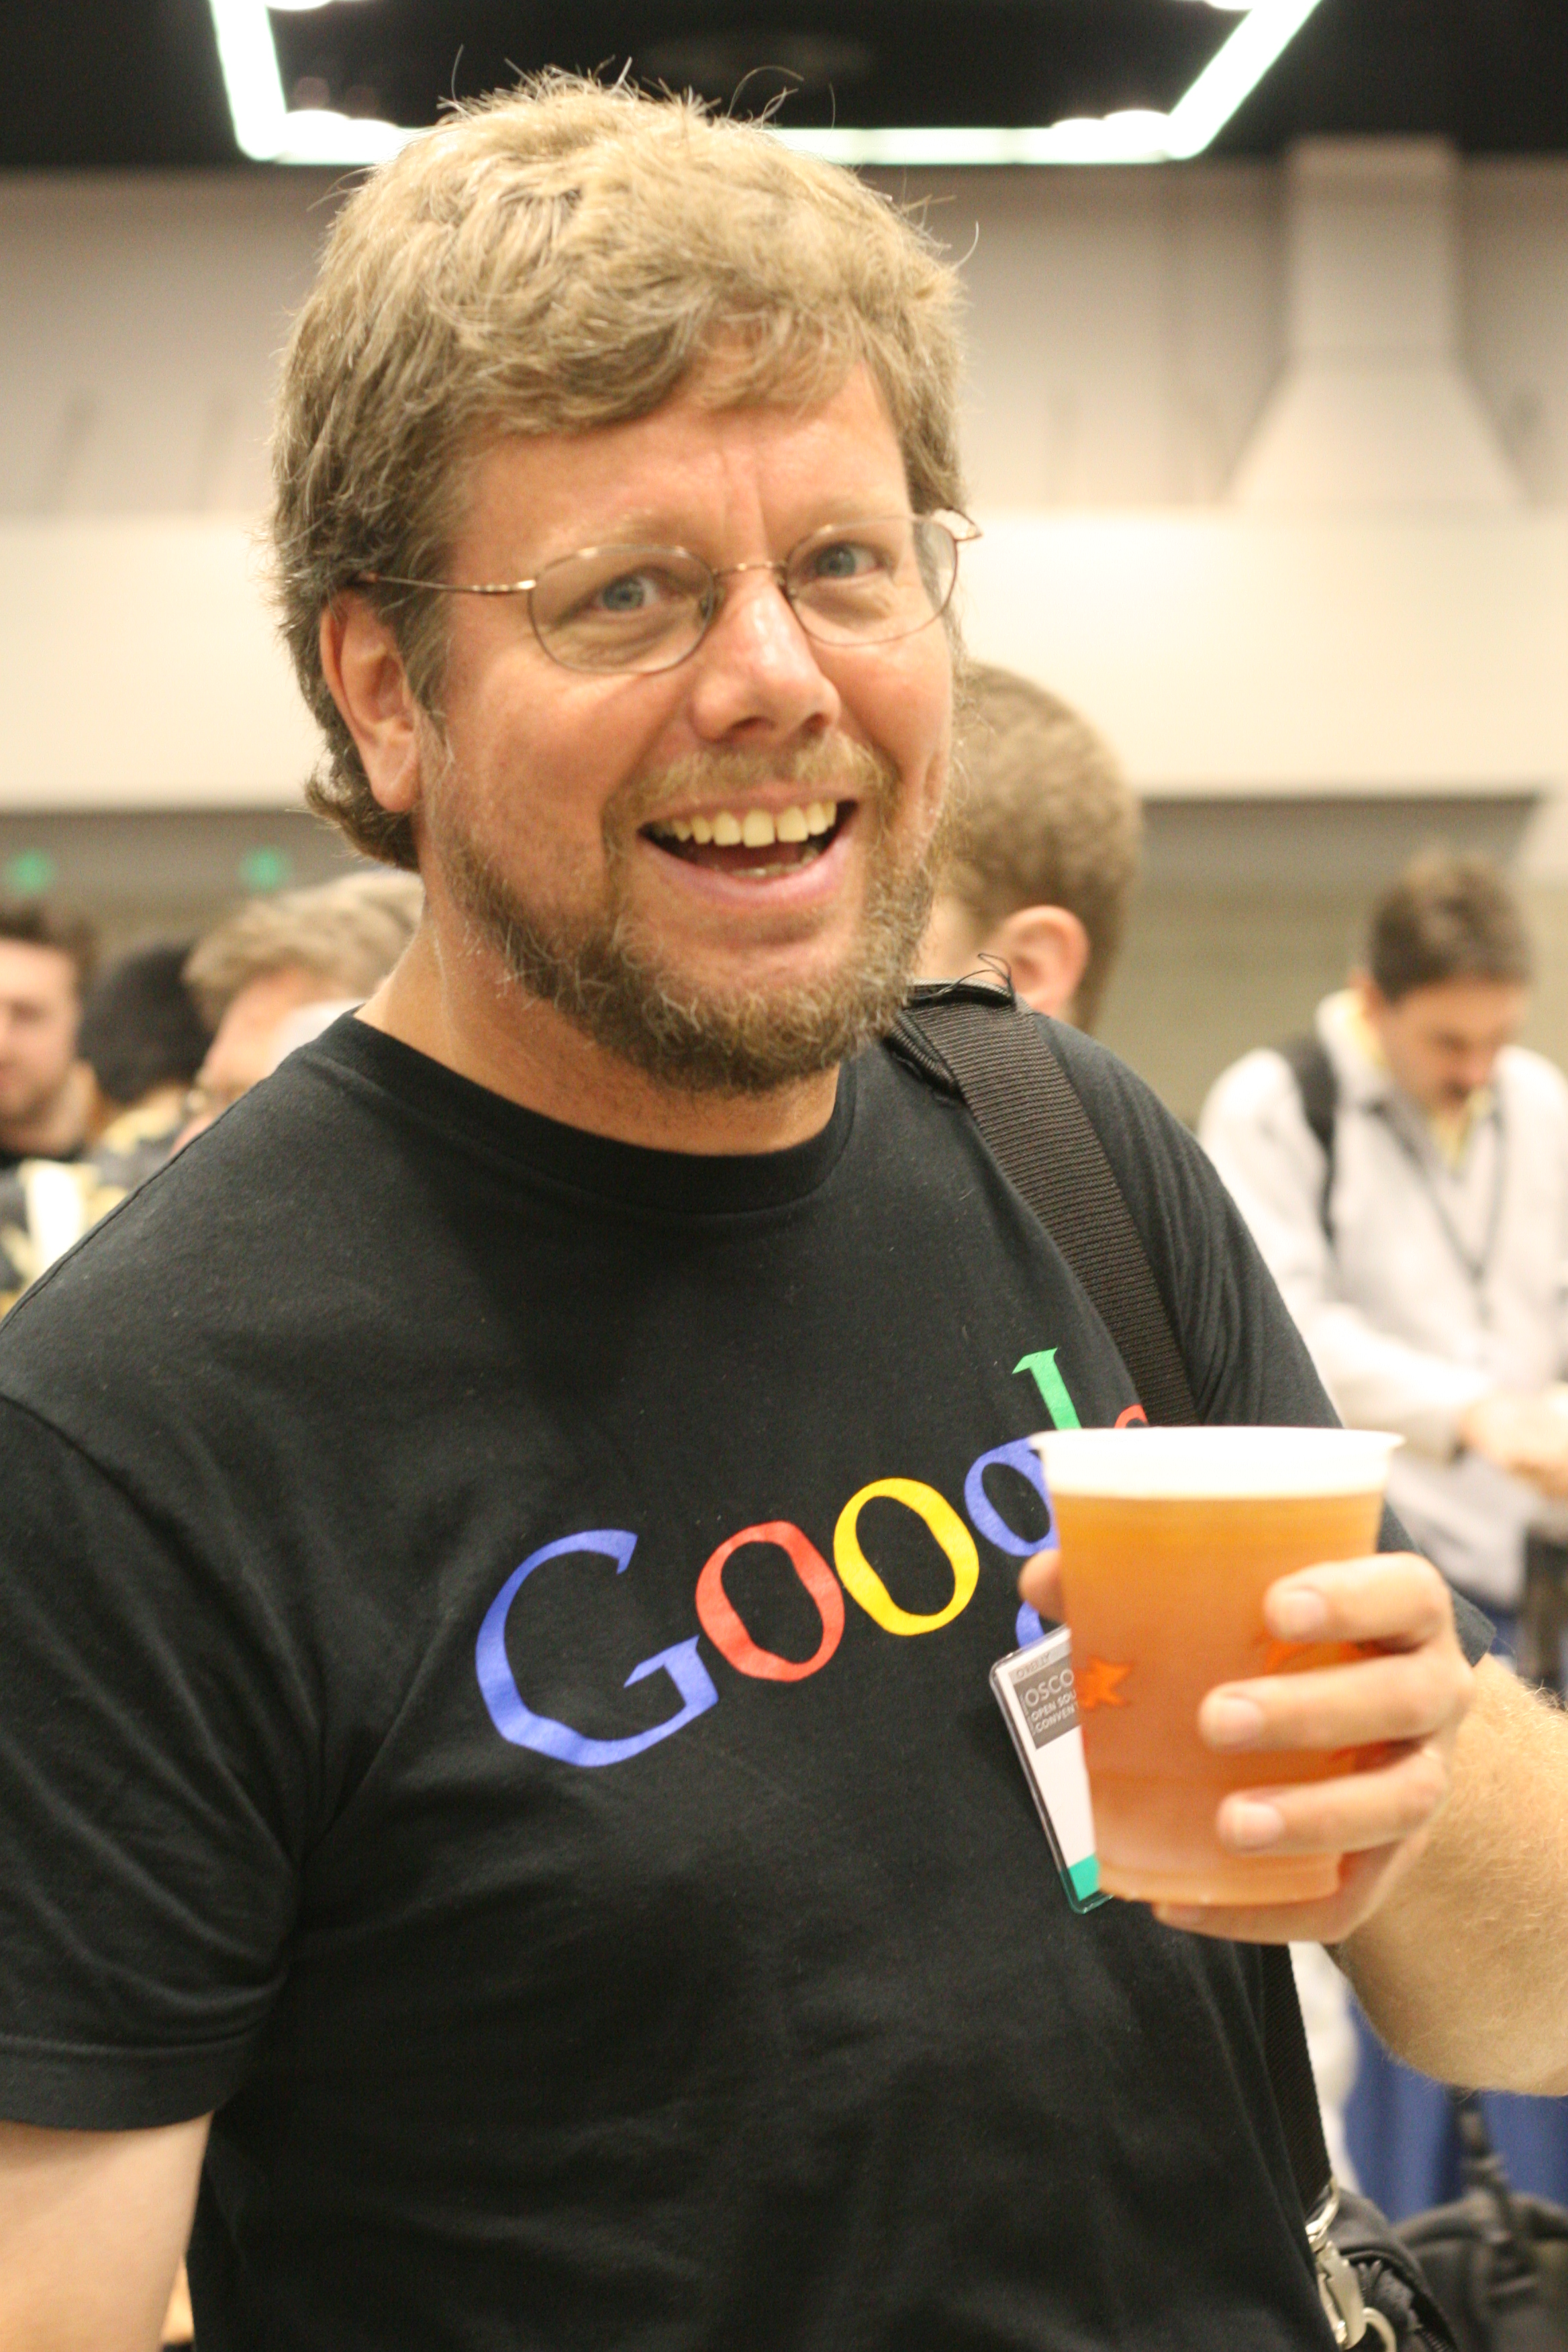
\includegraphics[width=0.4\textwidth]{pictures/1.jpg}
};
\end{tikzpicture}
	 	
		Guido van Rossum is a Dutch computer \\ 
 		programmer who is best known as the \\
 		author of the Python programming \\
 		language. In the Python community, \\
 		Van Rossum is known as a "Benevolent \\
 		Dictator For Life" (BDFL), meaning \\
 		that he continues to oversee the Python\\
 		development process, making decisions \\
 		where necessary.He was employed by \\
 		Google from 2005 until 7 December 2012,\\
 		where he spent half his time developing \\
 		the Python language. In January 2013, \\
 		Van Rossum started working for Dropbox.
\end{frame}
%-------------------------------------------------------
 		
%-------------------------------------------------------
\subsection{Versions}
\begin{frame}{Introduction}{Versions}
%-------------------------------------------------------	
\begin{block}{Python 1.0 | January 1994}
\begin{itemize}
	\item Python 1.6 - September 5, 2000
\end{itemize}
\end{block}	

\begin{block}{Python 2.0 | October 16, 2000}
	\begin{itemize}
		\item Python 2.7 - July 3, 2010
	\end{itemize}
\end{block}

\begin{block}{Python 3.0 | December 3, 2008}
	\begin{itemize}
		\item Python 3.5 - September 13, 2015
	\end{itemize}
\end{block}
\end{frame}
%-------------------------------------------------------
 		
 %-------------------------------------------------------
 \subsection{Installation}
 \begin{frame}{Introduction}{Installation}
 %-------------------------------------------------------
 		
 \url{https://www.python.org/downloads/}
 			
 \end{frame}
 %-------------------------------------------------------
 		

 		 
\defverbatim[colored]\interactivePython{
\begin{lstlisting}[numbers=left,language=Python,tabsize=4, showspaces=false]
>>> print("Hello, world")
\end{lstlisting}}

\defverbatim[colored]\scriptPython{
\begin{lstlisting}[numbers=left,language=Python,tabsize=4, showspaces=false]
#!/usr/bin/env python3
print("Hello, world")
\end{lstlisting}}
 		 
%-------------------------------------------------------
\subsection{Hello world!}
\begin{frame}{Introduction}{Hello world!}
%-------------------------------------------------------
\begin{block}{Interactive Python}
\interactivePython
\end{block}
\pause 		
\begin{block}{Script in Python}
\scriptPython
\end{block}

\end{frame}
%-------------------------------------------------------
 		
\defverbatim[colored]\keywordsPython{
\begin{lstlisting}[numbers=left,language=Python,tabsize=4, showspaces=false]
>>> import keyword
>>> print(keyword.kwlist)
\end{lstlisting}}	
%-------------------------------------------------------
\subsection{Python keywords}
\begin{frame}{Introduction}{Python keywords}
%-------------------------------------------------------
\begin{block}{Keywords}
 		
 	\begin{center}
	 		\begin{tabular}{| c | c | c | c | c |}
	 		\hline
	 		False & class & finally & is & return \\ \hline
	 		None & continue & for & lambda& try \\ \hline
	 		True & def & from & nonlocal & while \\ \hline
	 		and & del & global & not & with \\ \hline
	 		as & elif & if & or & yield \\ \hline
	 		assert & else & import & pass & break \\ \hline
	 		& except & in & raise & \\ \hline
	 		\end{tabular}
 	\end{center}
\end{block}
\pause
\begin{block}{Print all keywords}
	 \keywordsPython
\end{block}
 			
\end{frame}
%-------------------------------------------------------
\defverbatim[colored]\indentationPython{
\begin{lstlisting}[numbers=left,language=Python,tabsize=4, showspaces=true, showtabs=true]
if True:
    print("True")
else:
    print("False")

if True:
  print("True")
    print("Error")

if True:
    print("True")
	print("Error")
\end{lstlisting}}
%-------------------------------------------------------
\subsection{Indentation is very important!}
\begin{frame}{Introduction}{Indentation is very important!}
%-------------------------------------------------------	
 	\begin{block}{Indentation}
		\indentationPython
 	\end{block}	
 	
 		
\end{frame}
%-------------------------------------------------------
\defverbatim[colored]\quotesPython{
\begin{lstlisting}[numbers=left,language=Python,tabsize=4, showspaces=false]
word = 'word'
sentence = "This is a sentence."
paragraph = """This is a paragraph.
It is made up of multiple lines and sentences."""
Inside_1 = "Quotation 1 'inside'."
Inside_2 = 'Quotation 2 "inside".'
\end{lstlisting}}
%-------------------------------------------------------
\subsection{Quotes}
\begin{frame}{Introduction}{Quotes}
%-------------------------------------------------------	
\begin{block}{Quotes}
	\quotesPython
\end{block}
\end{frame}
%-------------------------------------------------------
\defverbatim[colored]\commentsPython{
\begin{lstlisting}[numbers=left,language=Python,tabsize=4, showspaces=false]
#!/usr/bin/python3
# First comment
print ("Hello, Python!") # second comment
\end{lstlisting}}
%-------------------------------------------------------
\subsection{Comments}
\begin{frame}{Introduction}{Comments}
%-------------------------------------------------------
\begin{block}{Comments}
	\commentsPython
\end{block}	
	
\end{frame}
%-------------------------------------------------------
\defverbatim[colored]\typesPython{
\begin{lstlisting}[numbers=left,language=Python,tabsize=4, showspaces=false]
#!/usr/bin/python3
counter = 100
miles = 1000.0
name = "John"
names = ["John", "Alex"]


print(counter, type(counter))
print(miles, type(miles))
print(name, type(name))
print(names, type(names))
\end{lstlisting}}
%-------------------------------------------------------
\subsection{Type of variables}
\begin{frame}{Introduction}{Type of variables}
%-------------------------------------------------------	
\begin{block}{Type of variables}
	\typesPython
\end{block}

\end{frame}
%-------------------------------------------------------

%-------------------------------------------------------
\begin{frame}{Introduction}{Questions?}
%-------------------------------------------------------
\large Questions?
\begin{center}
	
	\begin{block}{Contacts}
		\begin{itemize}
			\item email:    buzuma\_leha@mail.ru
			\item Facebook: aleksei.buzuma
		\end{itemize}
	\end{block}
		
\end{center}


\end{frame}
%-------------------------------------------------------

% Listing example without defverbatim tag
%\begin{frame}[fragile]
%	\frametitle{Source code}
%	
%	\begin{lstlisting}[caption=First C example]
%	int main()
%	{
%	printf("Hello World!");
%	return 0;
%	}
%	\end{lstlisting}
%\end{frame}
 		
\end{document}
 	